\documentclass[12pt, a4paper]{article}
\input{preamble}

\title{Surface scanning of Siegfried II in Gerdalinchen II}

\author{Jing Liu}

\date{\today{}}

\begin{document}
\maketitle{}
\tableofcontents

\section{Size of the beam spot}
\label{s:col}
The penetrating depth of 121~keV photons in tungsten is simulated
using MaGe:
\begin{lstlisting}
  $ MaGe ~/work/gerdalinchenII/scan/collimator/r2mm/W.mac
\end{lstlisting}
The 121~keV photons are emitted isotropically outward from the center
of a tungsten sphere. The geometry is defined in file
\lstinline!Wsphere.gdml! The radius of the hits ``hitR'' weighted by
their energy ``hitE'' are plotted in Fig.~\ref{f:w121}. Most of the
121~keV photons are stopped within 1~mm. The tungsten collimator used
in the scan can collimate the 121~keV photons almost perfectly. The
size of the beam spot on the surface of Siegfried~II can be calculated
geometrically. 

\begin{figure}[fptb]
  \centering
  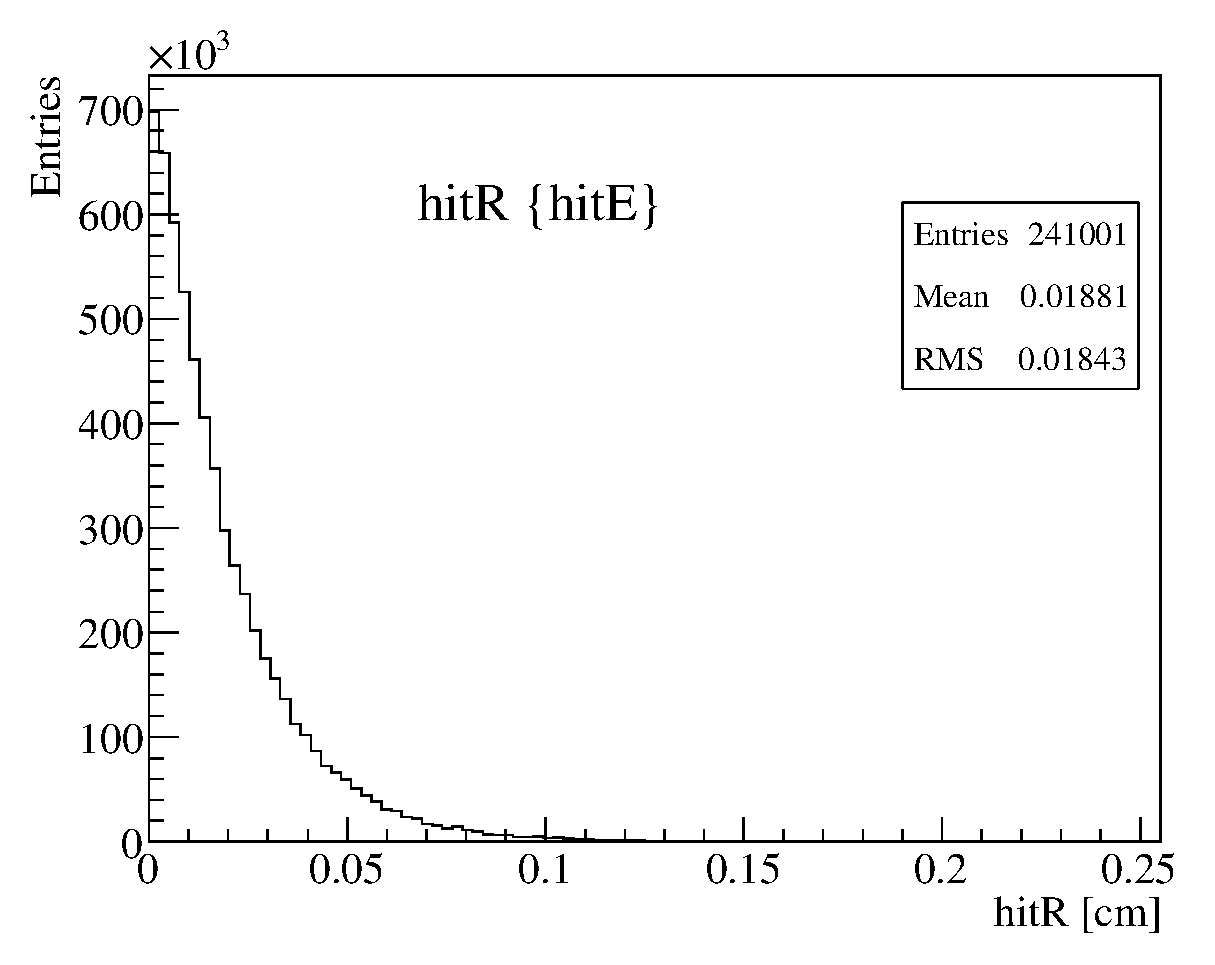
\includegraphics[width=0.5\textwidth]{w121keV}
  \caption{Penetrating depth of 121~keV photons in tungsten.}
  \label{f:w121}
\end{figure}

Figure~\ref{f:setup} showns the experimental setup. The diameter of
the beam spot $r$ on the surface of the detector can be calculated as:
\begin{equation}
  \label{e:size}
  r = (28+10.5)/28 \times 2 = 2.75 \text{ mm}.
\end{equation}

\begin{figure}[fptb]
  \centering
  \includegraphics[width=0.8\textwidth]{../../hole/occupancy/memo/segID}
  \caption{Experimental setup.}
  \label{f:setup}
\end{figure}

\end{document}

%%% Local Variables:
%%% mode: latex
%%% TeX-master: t
%%% End: 
